\section{Dataset generation}
\subsection{Tested approaches}
The deep learning approaches explained in this document are \textit{supervised learning} techniques that require a labeled dataset. Several paths were tested in order to generate this kind of dataset:
\begin{itemize}
    \item \emph{IMU sensors}: usage of gyroscope and accelerometer sensors of a smartphone to estimate the position of the camera during a video given a fixed origin point. 
    \item \emph{digital video}: usage of free online 3 dimensional datasets in which video can be recorder in a digital way.
    \item \emph{motion capture system}: usage of a motion capture system that estimates the camera position following some tracking objects attached to the subject.
    \item \emph{structure from motion techniques}: techniques that compute a sparse and dense reconstruction from a sequence of images.
\end{itemize}

The main problem encountered with IMU sensors was the high noise presence during acquisitions, the final signal was very dirty, and the resolution was not acceptable for the dataset generation. A possible solution could have been the usage of a well calibrated hardware used in other kind of contexts.

Most of the 3 dimensional acquisitions available online for free are acquired with \emph{depth sensors} or \emph{LIDAR sensors}, for this reason although the camera pose estimation would not have presented any errors the images would have been at low quality.

The motion capture system is able to follows the position of the tracked objects with extremely precision, the main problematic remains the association of poses to video captured from the camera held by the tracked subject. Other difficulties involved the calibration of the tool.

The techniques of structure from motion were invented with the goal of generate structures for which a huge amount of photos is available. The overall idea is to feed the algorithm with data in order to extract feature and build a recomposition of the environment. A step required in order to obtain a result is the estimation of the pose of images. These intermediate requirement have been exploited by us to generate a labeled dataset.

\subsection{Pipeline}
The implemented pipeline require a video captured by any camera, it is not required any calibration of the sensor. It is composed by several steps:
\begin{enumerate}
    \item video split: the captured video is split into many frames; 
    \item structure from motion: images obtained from the previous step are fed into a structure motion tool called \emph{COLMAP};
    \item cross validation dataset: positions obtained during the camera estimation of the reconstruction process are split into three batches: train, validation, test.
\end{enumerate}

\begin{figure}[h]
    \begin{center}
        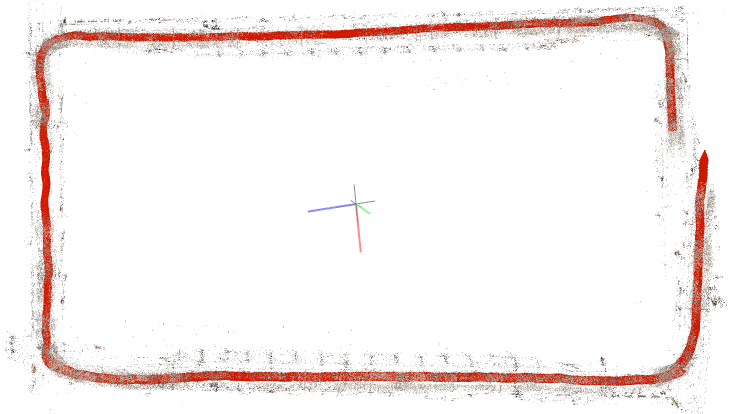
\includegraphics[width=0.45\textwidth]{./imgs/trajectory_colmap.png}
    \end{center}
    \caption{Trajectory computed by COLMAP}
    \label{fig:trajectory-colmap}
\end{figure}

In \cref{fig:trajectory-colmap} is presented the trajectory obtained with the structure from motion techinque through COLMAP. The process involes a feature extraction phase.

\subsection{COLMAP reconstruction}
COLMAP~\cite{colmap} is a tool that allows to build a 3D reconstruction (model) of an environment. There exists two types of models, \textit{sparse} and \textit{dense} and both of them are composed by:
\begin{itemize}
    \item a set of points $P$ which are features of the environment (dots on \cref{fig:features-colmap});
    \item a set of poses $\mathcal{V}$ associated witht the images used for the reconstruction (red squares on \cref{fig:features-colmap});
    \item a Coordinate Reference system.
\end{itemize}

\begin{figure}[h]
    \begin{center}
        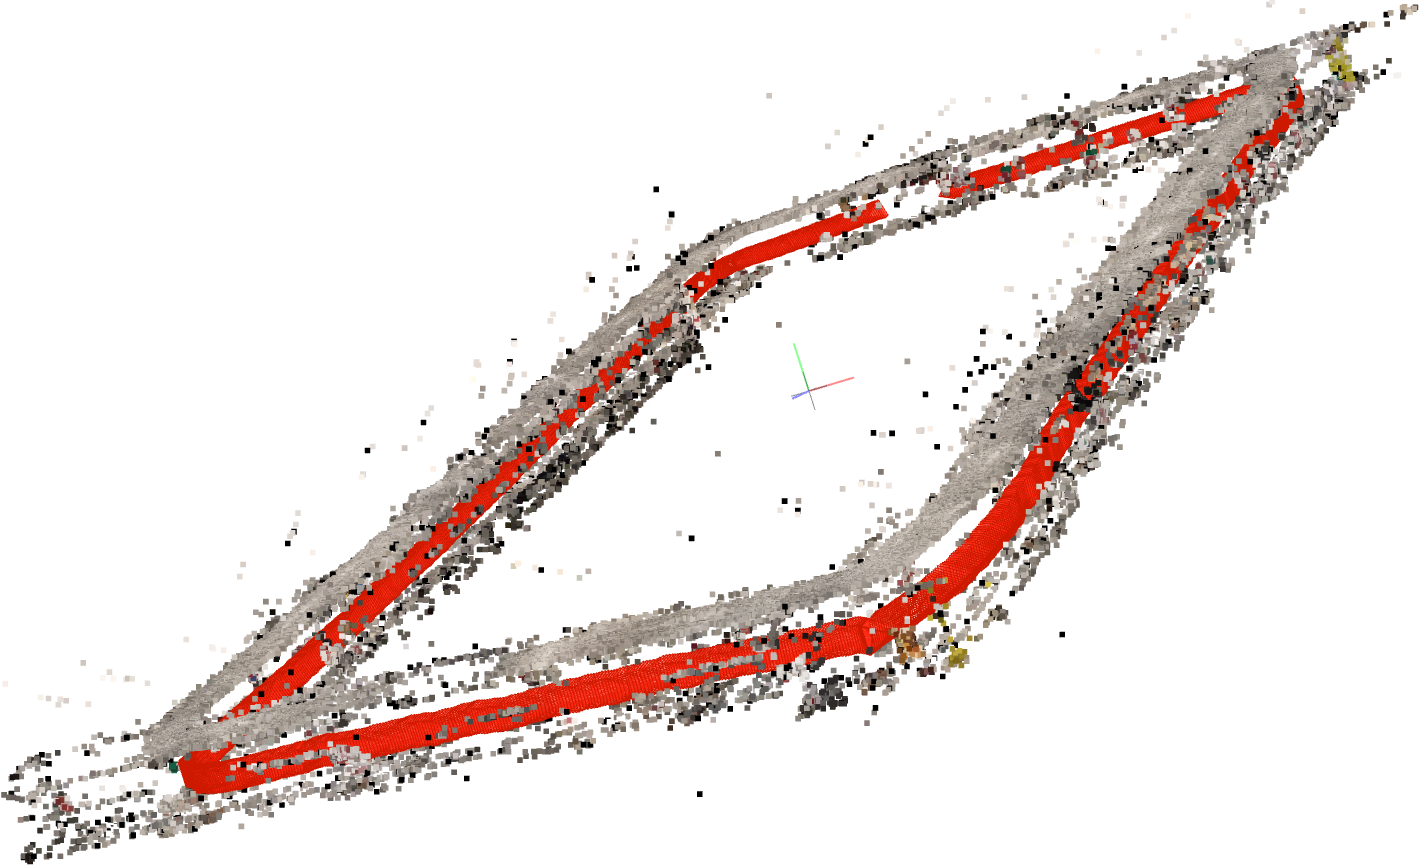
\includegraphics[width=0.45\textwidth]{./imgs/extracted_features_colmap.png}
    \end{center}
    \caption{Features extracted by COLMAP}
    \label{fig:features-colmap}
\end{figure}

The set of poses are represented as a graph $\mathcal{G}=(\mathcal{V}, \mathcal{E})$ and for each node there is an association with a subset of environment features $\mathcal{V} = \{R\}\quad R\subset P$. Edges $\mathcal{E}$ connect following poses.

The algorithm that creates a sparse model extracts features from each given image and build the set $P$ called \textit{bag of words}. Once this is done, thanks to a convolution on each image, the next step is to created associations between node of the graph. The convolution enables to map only subsection of the whole image, this allows to estimate the movement based on the position of the matrix used for the convolution within the image grid. The bag of words is consulted at every step. Once associations are done the features and the poses are composed in order to create the sparse model.

The algorithm for the dense model is very similar to the one used for the sparse. Tha main differences is how the association are created, it is not used a convolution but a pointwise method. This allows to be more accurate and create a more definite cloud of points increasing the computational time.

The settings used for sparse dataset generation of Povo 1 used a sequence of images with Poisson mesher.

\subsection{Coordinate reference system alignment}
The dataset generated by COLMAP has a \textit{coordinate reference system (CRS)} choosen arbitrarily during the reconstruction. Origin and axes of the system may not concide with the real world CRS. In order to be able to place a prediction on a map it is required to rotate and translate until an alignment is reached.

This task was accomplished through the Euclidean or Rigid transformation, it invoves a rotation $R$, a translation $t$ and at least three points for both the CRSs that represents the same locations $A=\{(x_1^A, y_1^A), (x_2^A, y_2^A), (x_3^A, y_3^A)\}$, $B=\{(x_1^B, y_1^B), (x_2^B, y_2^B), (x_3^B, y_3^B)\}$. In \cref{eq:rigid-tranform} is presented the equation of the rigid transform.
\begin{equation}
    R\times A+t = B
    \label{eq:rigid-tranform}
\end{equation}

Matrix $R$ and vector $t$ are obtained using \textit{Singular value decomposition (SVD)}, it takes a matrix $E$ and return 3 other matrices, such that: 
\begin{equation}
    \begin{aligned}
        [U, S, V] &= SVD(E)\\
        E &= USV^T
    \end{aligned}
    \label{eq:singular-value-decomposition}
\end{equation}

The first step needed to extract the matrix $R$ is the alignment on the same origin of the datasets centroids. This is done subtracting to each coordinate of each point the centroid of the dataset. Once this is done it is possible to ignore the component of the translation $t$ and compute the rotation $R$:
\begin{equation}
    \begin{aligned}
        H &=(A-\text{centroid}_A)(B-\text{centroid}_B)^T\\
        [U, S, V] &= SVD(H)\\
        R &=VU^T
    \end{aligned}
    \label{eq:rotation-matrix}
\end{equation}

Finally it is possible to use the \cref{eq:rigid-tranform} to obtain the translation vector $t$:
\begin{equation}
    \begin{aligned}
        R\times A + T &= B\\
        R\times \text{centroid}_A + T &= \text{centroid}_B\\
        t &= \text{centroid}_B - R\times \text{centroid}_A
    \end{aligned}
    \label{eq:translation-vector}
\end{equation}
